\chapter{APPENDIX}
%\setcounter{section}{A}
\begingroup
\let\clearpage\relax
\phantomsection
\addcontentsline{toc}{section}{\protect\numberline{}\textbf{Appendix A:} Mathematical Model}%
\chapter*{A: MATHEMATICAL MODEL}
\endgroup
The relationship between files and tags can be represented by using Set theory. Set theory is the branch of mathematics that studies sets, which are collections of objects. The following mathematical model represents the working of this filesystem. 

\noindent The following dynamic and variable sets are defined as, \\
\indent $F$	: Set of Files \\
\indent $T$	: Set of Tags \\
\indent $S$	: Set of Tags in query ( $S \subseteq T$ ) \\

\subsection{Relation between Files (F) and Tags (T)}
$$ R = \{(f,t) \mid f \,\, has \,\, tag \,\,t; f \in F, t \in T\}$$
Here $R$ defines the relation between a file $f$ and its tag $t$ where $R \subseteq F \times T$. This relationship is \emph{many-to-many}. 
That is a file can have many tags, and a tag can describe many files.

\subsection{Association between Tags (T)}
Using discovered associations, we can form various relations between tags. These \emph{tag-to-tag} help in displaying related information. For any two tags there exists a distinct relation between them given by $r$. The function $X_{r}(A,B)$ returns the relation between two tags. Associations can be broadly categorized as:
\begin{itemize}
\item {$A \sim B$} : $A$ and $B$ are not directly related, but there \emph{may} exist some indirect relation between them.
\item $A \succ B$ : $A$ and $B$ are directly related, where $A$ always has a path leading to $B$. This relation is similar to $A \subset B$.
\item $A \bowtie B$ : $A$ and $B$ are not directly related, but $B$ supplements additional information related to $A$.
\item $\phi$ : This relation states that there does not exist any relation between the two tags.
\end{itemize}

\subsection{Operations}
$$g(f) = \{t : f \, R \, t\}$$
$g$ is an operation which takes input as a file $f$ and returns the set of tags ($t \in S$) related by $R$ to that file.

$$h(t) = \{f : f \, R \, t\}$$
$h$ is an operation which takes input as a tag $t$ and returns the set of files ($f \in F_{S}$) related by $R$ to that tag.

%----------------------------------------------------------------------------------------------------------------------------------

\subsection{Storing Tags and Files}
The relation $R$ is stored as a set of ordered pairs $(f,t)$, where $R \subseteq F \times T$. The operations $g$ and $h$ operate on these ordered pairs and return mapped or matched elements. A relation which has to be added must be represented in the form of of ordered pair $(f,t)$. Storage of all relations is given by $F \times T$ where ordered pairs exist according to $R = \{f \in F, t \in T \mid f\, R \,t\}$.

\noindent For example, we have the sets and their relations as: 
$$F = \{ f_{1}, f_{2}, f_{3} \}, T = \{ t_{1}, t_{2}, t_{3} \}, R = \{f_{1} \, R  \, t_{1}, f_{2}  \, R  \, t_{2}, f_{3}  \, R  \, t_{1}, f_{1}  \, R  \, t_{3}\}$$
Then we store this relation by its ordered pairs given by:
$$R = \{(f_{1},t_{1}),(f_{2}, t_{2}),(f_{3}, t_{1}),(f_{1}, t_{3})\}$$

\subsection{Extraction of metadata}
The extraction of metadata is defined by the function $X_{E}$ which takes a file $f(f \in F)$ and returns a set of tags $(T_{E} \subseteq T)$ that form the relation ($f  \, R  \, t : t \in T_{E}$). 
$$X_{E}(f) = T_{E} \in 2^{T}$$

\noindent Addition of new information (metadata, tags) is done as:
$${if (t \notin T) \, then \, (T \gets T \cup \{t\})}$$

\noindent We then store this relation as a ordered pair $\{(f, \, t) \, \forall t \in T_{E}\}$. At the end of this operation $T_{E} \subseteq T$ will hold true. 

\subsection{Importing Semantics}
The existing file-directory structure can be imported to the system and represented in the form of tags and files. We define: 

\noindent $F_{H} \, $  : Set of \emph{Files} on hard-disk which are not represented in system.\\
$D_{H}$ : Set of \emph{Directories} on hard-disk which are not represented in system. \\

\noindent Then for every file stored within a directory $d$, the relation $R$ is expressed as 
$(f  \, R  \, d)$.
When importing semantics we create the ordered pair $(f,d)$ given by the relation $(f  \, R \,  d, \forall d \in D_{d})$. Where $D_{d}$ contains the directory the file is stored in, as well as every parent directory of that directory itself.

\noindent Directories also contain sub-directories which we store in the form of tag relationships. We represent them as:
$\forall (d_{1}, d_{2}) \in D_{H}$, if $d_{2} \subset d_{1}$ ($d_{2}$ is a sub-directory of $d_{1}$) store the relation as
$$d_{1} \to d_{2}$$


\subsection{Apriori Algorithm}
The apriori algorithm\cite{FastAlgo} is a classic algorithm for learning association rules. The
 algorithm is designed to operate on databases containing transactions. As is
common in association rule mining, given a set of itemsets (for instance, sets
of retail transactions, each listing individual items purchased), the algorithm
attempts to find subsets which are common to at least a minimum number C of the
itemsets. Apriori uses a "bottom up" approach, where frequent subsets are
extended one item at a time (a step known as candidate generation), and groups
of candidates are tested against the data. The algorithm terminates when no
further successful extensions are found.

The purpose of the apriori algorithm is to find associations between different sets of data.
Each set of data has a number of items and is called a transaction.
The output of Apriori is sets of rules that tell us how often items are contained in sets of data.

\subsubsection{Itemset}
A collection of one or more items. \\
Example: {A, B, C} \\ \\
\textbf{k-itemset} \\
An itemset that contains k items.

\subsubsection{Support count (S)}
Number of transactions containing an itemset. \\
Example: S({A, B}) = 2

\subsubsection{Support (supp)}
The support supp(X) of an itemset X is defined as the proportion of transactions in the data set which contain the itemset.
Suppose \textit{minsup} is the minimum support threshold.
Example: supp({A, B}) = 2/5

\subsubsection{Frequent Itemset (L)}
An itemset satisfies minimum support if the occurrence frequency of the itemset
is greater or equal to a threshold. If an itemset satisfies minimum support, then it is a frequent itemset.
Thus an itemset whose support is greater or equal to minsup is a frequent itemset.

\subsubsection{Confidence}
The confidence of a rule is defined as,\\
\begin{equation}
Conf(A \rightarrow B) = supp(A \rightarrow  B) / supp(A)
\end{equation}
Suppose \textit{minconf} is the minimum confidence threshold.

\subsubsection{Rule Generation}
Given a set of transactions T, the goal of association rule mining is to find all rules having\\
\begin{equation}
support \geq minsup \; threshold
\end{equation}
\begin{equation}
confidence \geq minconf \; threshold
\end{equation}

Given a frequent itemset L, find all non-empty subsets $f \subset L$ such that $f \rightarrow  L - f$ satisfies the minimum confidence requirement.

Example: If ${A, B, C}$ is a frequent itemset, then the following candidate rules are formed \\
${ AB \rightarrow  C, \; AC \rightarrow  B, \; BC \rightarrow  A, \; A \rightarrow  BC, \; B \rightarrow  AC, \; C \rightarrow  AB }$ 

If $|L| = k$, then there are $(2 ^ k) - 2$ candidate association rules 
$(ignoring \,\; L \rightarrow \Phi \; and \;\; \Phi \rightarrow L)$

\subsubsection{Apriori principle}
The princciple sttes that if an itemset is frequent, then all of its subsets must also be frequent.
Apriori principle holds due to the following property of the support measure:
\begin{equation}
\forall X , Y : ( X \subseteq Y ) \rightarrow  s( X ) \geq s(Y )
\end{equation}

Support of an itemset never exceeds the support of its subsets. This is known as the anti-monotone property of support.

$\newline$
\textbf{Algorithm} \\
Input \\
T - Database of transactions \\
I   - Items \\
L - Itemset\\
s   - support\\
c - confidence

$\newline$
Output \\
R - Association rules satisfying s and c

$\newline$
Algorithm to Generate Frequent Itemsets\\
Apriori(T,s)\\
$L_{1} \leftarrow {Large \; 1-itemset} \\
k \leftarrow 2 \\
while \; L_{k - 1} \neq \Phi \\
C_{k} = Generate(L_{k - 1}) \\
	for \;  transactions  t \in T \\
		C_{t} \leftarrow Subset(C_{k}, t) \\
		for \; candidates \; c \in C_{t} \\
			count[c] \leftarrow \; count[c] + 1 \\
		L_{k} \leftarrow {c \in C_{k} | count[c] \geq s} \\
		k \leftarrow k + 1 \\
return \cup L_{k}$

$\newline$
Algorithm to Generate Association Rules\\
GenRule\\
$R = \Phi;\\
	for \; each \; l \in L \; do \\
		for \; each \; x \subset l \; such \; that \; x \neq \Phi \; and \; x \neq l \; do \\ 
			if (supp(l) \; / \; supp(x)) \geq c \; then \\
				R = R \; \cup \; ( x \rightarrow ( l - x ) )$;
				
				
				
\newpage				
\setcounter{subsection}{1}
\setcounter{subsubsection}{1}
\phantomsection
\addcontentsline{toc}{section}{\protect\numberline{}\textbf{Appendix B:} Testing of Data}
\chapter*{B: TESTING OF DATA}

Testing of the system will be done on the following points:

\subsection{Storing the relation $R$:}
The working of the system depends on correctly storing the relation $R$. These tests check whether the relations are stored and represented correctly. 
\begin{enumerate}
\item For any file $f$ associated with tag $t$ there should exist an ordered pair $(f,t)$.
\item For a file $f$ associated with tags $S = \{t_{1}, t_{2}, t_{3}\}$, the operation $g(f)$ should return exacty $S$.
\item For a tag $t$ containing files $F = \{f_{1}, f_{2}, f_{3}\}$, the operation $h(t)$ should return exactly $F$.
\end{enumerate}

\subsection{Relation between tags: }
\begin{enumerate}
\item The relation $r$ between two tags $t_{1},t_{2}$ is given by function $X_{r}(t_{1},t_{2})=c$.
\item The relation $r$ is distinct i.e. there exists only one relation between any two tags. If contradictions arise where more than one relation is present between two tags, then all those relations must be made void and $r=\phi$. The user can then explicitly specify which relation should be created between those two tags.
\item Extensive testing must be done on relations to determine which $r$ needs to be set under certain conditions.
\end{enumerate}

\subsection{Extraction of Metadata:}
Let $M$ be the set of all metadata tags $t$ for file $f$. The function $X_{E}$ represents an algorithm to extract t from f. It returns a set $T_{E}$ such that $\{t \in T_{E} \mid f \, R \, t\}$ and $(T_E \subseteq M)$. To test the efficiency of the function, or the effectiveness of it, we compare the cardinality of the generated set $T_E$ with the set of Metadata $M$. The efficiency can be calculated by
$$\mathrm{Efficiency} \, \epsilon = \frac {\mid T_E \mid} {\mid M \mid}$$
Using $\epsilon$ we can compare algorithms and their efficiency. Appropriate algorithms can be chosen for various file types so that efficiency of the entire system remains high. For e.g. \\
\indent $X_{E1} : \{\epsilon =0.7$ for audio$, \epsilon = 0.4$ for images $\}$ \\
\indent $X_{E2} : \{\epsilon =0.6$ for audio$, \epsilon = 0.6$ for images $\}$ \\
Then we have the following options:
\begin{enumerate}
\item $X_{E2}$ is a better choice as it yeilds a more consisten efficiency.
\item $X_{E1}$ is used only for audio and $X_{E2}$ is used only for image extractions.
\end{enumerate}


\subsection{Queries and their results:}
Queries are parsed into tokens of the form $(t_1, \sigma , t_2)$. We need to test whether $\sigma $ returns the correct results for the query. A Query $Q(S)$ is said to be successfully executed when the expected result are shown.  
\begin{itemize}
\item The Query $q(t)$ for a single tag $t$ should return a set of files $(f \in F_{S})$ through the operation $h(t)$. 
\item In a query if no operation is given, Intersubsection should be performed. 
\item For Query $Q(S)$ the operations should be performed from left to right unless precedence is specified by paranthesis. 
\end{itemize}

Example:
\noindent Let $t_{1}, t_{2}, t_{3}$ be tags having the following files: \\
\indent $t_{1}$ : $\{photo_{1},photo_{2},doc_{1}\}$  \\
\indent $t_{2}$ : $\{photo_{1},doc_{1}, ppt_{1}\}$  \\
\indent $t_{3}$ : $\{photo_{1},doc_{3}\}$ 
\begin{enumerate}
\item $q(t) = F_{S}$ where $f$ should follow the relation $(f \in F_S \mid f \, R \, T)$. 
For example, q$(t_{1})$ returns $F_S = \{photo_{1},photo_{2},doc_{1}\}$.
\item Consider a query containing tags $S = \{t_{1}, t_{2}\}$. 
It generates results by performing the operations $Q(S) = q(t_{1})\sigma q(t_{2})$
where $\sigma $ is an operator.
\begin{enumerate}
\item Putting $\sigma = \cup$ for Union in query $Q(S) = q(t_{1})\cup q(t_{2})$; the result should be $F_S = \{photo_1, photo_2, doc_1, ppt_1\}$. 	
\item Putting $\sigma = \cap$ for Intersubsection in query $Q(S) = q(t_{1})\cap q(t_{2})$; the result should be $F_S = \{photo_1, doc_1\}$.
\item Putting $\sigma = \setminus$ for Set Difference in query $Q(S) = q(t_{1})\setminus q(t_{2})$; the result should be $F_S = \{photo_2\}$, whereas the query $Q(S) = q(t_{2}) \setminus q(t_{1})$ will return the result as $F_S = \{ppt_1\}$.
\item Putting $\sigma = \ominus$ for Symmetric Difference in query $Q(S) = q(t_{1})\ominus q(t_{2})$; the result should be $F_S = \{photo_2, ppt_1\}$.
\end{enumerate}

\item Consider a query containing tags $S = \{t_{1}, t_{2}, t_{3}\}$.
It performs operations as : $Q(S) = q(t_{1})\sigma_{1} q(t_{2})\sigma_{2} q(t_{3})$
The default order for processing is from left to right unless precedence is specified through parenthesis.

\begin{enumerate}
\item For the query $Q(S) = q(t_{1}) q(t_{2}) q(t_{3})$ the result will be returned as files $\{photo_{1}\}$
\item For the query $Q(S) = q(t_{1}) \cup q(t_{2}) \cap q(t_{3})$ the result will be returned as files $\{photo_{1}, doc_{1}, doc_{3}\}$
\end{enumerate}
\end{enumerate}

After verifying that individual queries return correct results, we must check whether $Q(S)$ runs correctly as well. This is done by seperating the query into tokens, and calculating their results in turn. It must be verified that results are correct and have not been mis-intepreted through tokenization of the query.
%----------------------------------------------------------------------------------------------------------------------------------------

\subsection{Forming Associations}
Consider a database, D, consisting of 9 transactions.
Suppose minimum support count required is 2 (i.e. $minsup = 2 / 9 = 22\%$ ).
Let minimum confidence required is $minconf = 70\%$.
We have to first find out the frequent itemset using apriori algorithm.
Then, Association rules will be generated using minsup and minconf.

\begin{center}
\begin{tabular}{|l|l|}
\hline
\textbf {TagID} & \textbf {Files} \\ \hline
T100 & F1, F2, F5  \\ \hline
T101 & F1, F2, F5  \\ \hline
T102 & F2, F4  \\ \hline
T103 & F2, F3  \\ \hline
T104 & F1, F2, F4  \\ \hline
T105 & F1, F3  \\ \hline
T106 & F2, F3  \\ \hline
T107 & F1, F3  \\ \hline
T108 & F1, F2, F3, F5  \\ \hline
T109 & F1, F2, F3  \\ \hline
\end{tabular}
\end{center}

$\newline$
\textbf{Step 1: Generating initial Candidate Itemset} \\
In the first iteration of the algorithm, each item is a member of the set of candidate.

\begin{center}
\begin{tabular}{|l|l|}
\hline
\textbf {Itemset} & \textbf {Support count} \\ \hline
\{F1\} & 6  \\ \hline
\{F2\} & 7  \\ \hline
\{F3\} & 6  \\ \hline
\{F4\} & 2  \\ \hline
\{F5\} & 2  \\ \hline
\end{tabular}
\end{center}

$\newline$
\textbf{Step 2: Generating 1-itemset Frequent Pattern} \\
The set of frequent 1-itemsets, L1, consists of the candidate 1-itemsets satisfying minimum support.

\begin{center}
\begin{tabular}{|l|l|}
\hline
\textbf {Itemset} & \textbf {Support count} \\ \hline
\{F1\} & 6  \\ \hline
\{F2\} & 7  \\ \hline
\{F3\} & 6  \\ \hline
\{F4\} & 2  \\ \hline
\{F5\} & 2  \\ \hline
\end{tabular}
\end{center}

$\newline$
\textbf{Step 3: Generating 2-itemset Frequent Pattern} \\
To discover the set of frequent 2-itemsets, L2, the algorithm uses L1 Join L1 to generate a candidate set of 2-itemsets, C2.
Next, the transactions in D are scanned and the support count for each candidate itemset in C2 is accumulated.
The set of frequent 2-itemsets, L2, is then determined, consisting of those candidate 2-itemsets in C2 having minimum support.

\begin{center}
\begin{tabular}{|l|l|}
\hline
\textbf {Itemset} & \textbf {Support count} \\ \hline
\{F1, F2\} & 4  \\ \hline
\{F1, F3\} & 4  \\ \hline
\{F1, F5\} & 2  \\ \hline
\{F2, F3\} & 4  \\ \hline
\{F2, F4\} & 2  \\ \hline
\{F2, F5\} & 2  \\ \hline
\end{tabular}
\end{center}

$\newline$
\textbf{Step 4: Generating 3-itemset Frequent Pattern}\\
The generation of the set of candidate 3-itemsets, C3, involves use of the Apriori Property. First, we generate C3 using L2 join L2. \\
\begin{center}
C3 = \{\{F1, F2, F3\}, \{F1, F2, F5\}, \{F1, F3, F5\}, \\
\{F2, F3, F4\}, \{F2, F3, F5\}, \{F2, F4, F5\}\}.
\end{center}
Now we will apply Apriori property to determine which candidate itemsets are frequent.

The 2-item subsets of \{F1, F2, F3\} are \{F1, F2\}, \{F1, F3\} and \{F2, F3\}.
Since all 2-item subsets of \{F1, F2, F3\} are members of L2, We will keep \{F1, F2, F3\} in C3.

The 2-item subsets of \{F2, F3, F5\} are \{F2, F3\}, \{F2, F5\} and \{F3, F5\}.
But, \{F3, F5\} is not a member of L2 and hence it is violating Apriori Property.
Thus we will remove \{F2, F3, F5\} from C3.
Therefore,
\begin{center}
C3 = \{\{F1, F2, F3\}, \{F1, F2, F5\}\}.
\end{center}
Now, the transactions in D are scanned in order to determine L3, consisting
of those candidates 3-itemsets in C3 having minimum support.

\begin{center}
\begin{tabular}{|l|l|}
\hline
\textbf {Itemset} & \textbf {Support count} \\ \hline
\{F1, F2, F3\} & 2  \\ \hline
\{F1, F2, F5\} & 2  \\ \hline
\end{tabular}
\end{center}

$\newline$
\textbf{Step 5: Generating 4-itemset Frequent Pattern}\\
The algorithm uses L3 Join L3 to generate a candidate set of 4-itemsets, C4.
Although the join results in \{\{F1, F2, F3, F5\}\}, this itemset is removed since its subset \{\{F2, F3, F5\}\} is not frequent.
Thus, $ C4 = \Phi $ , and algorithm terminates, having found all of the frequent items.
This completes our apriori algorithm.

$\newline$
\textbf{Step 6: Generating Association Rules from Frequent Itemsets} \\
For each frequent itemset 'l', generate all nonempty subsets of l.
For every nonempty subset s of l, output the rule $ s \rightarrow  (l-s) $ if $ supp(l) \; / \; supp(s) \geq minconf $

We had L = \{\{F1\}, \{F2\}, \{F3\}, \{F4\}, \{F5\}, \{F1, F2\}, \{F1, F3\}, \{F1, F5\}, \{F2, F3\}, \{F2, F4\}, \{F2, F5\}, \{F1, F2, F3\}, \{F1, F2, F5\}\}.

Consider l = \{F1, F2, F5\}. Its all nonempty subsets are \{F1, F2\}, \{F1, F5\}, \{F2, F5\}, \{F1\}, \{F2\}, \{F5\}.

The association rules are shown below, each listed with its confidence.
\begin{enumerate}
\item $R1: F1, F2 \rightarrow F5 \\
Confidence = supp\{F1, F2, F5\} / supp\{F1, F2\} = 2 / 4 = 50 \% $ \\
R1 is Rejected.
\item $R2: F1, F5 \rightarrow F2$\\
$Confidence = supp\{F1, F2, F5\} / supp\{F1, F5\} = 2 / 2 = 100 \% $\\
R2 is Selected.
\item $R3: F2, F5 \rightarrow F1$\\
$Confidence = supp\{F1, F2, F5\} / supp\{F2, F5\} = 2 / 2 = 100 \% $\\
R3 is Selected.
\item $R4: F1 \rightarrow F2, F5$\\
$Confidence = supp\{F1, F2, F5\} / supp\{F1\} = 2 / 6 = 33 \% $\\
R4 is Rejected.
\item $R5: F2 \rightarrow F1, F5$\\
$Confidence = supp\{F1, F2, F5\} / supp\{F2\} = 2 / 7 = 29 \% $\\
R5 is Rejected.
\item $R6: F5 \rightarrow F1, F2$\\
$Confidence = supp\{F1, F2, F5\} / supp\{F5\} = 2 / 2 = 100 \% $\\
R6 is Selected.
\end{enumerate}

In this way, we have found the following three strong association rules.
\begin{enumerate}
\item $F1, F5 \rightarrow  F2$
\item $F2, F5 \rightarrow  F1$
\item $F5 \rightarrow  F1, F2$
\end{enumerate}

%\newpage
%\input{testingofdata.tex}
\newpage
%\setcounter{section}{A}
\setcounter{subsection}{1}
\setcounter{subsubsection}{1}
\phantomsection
\addcontentsline{toc}{section}{\protect\numberline{}\textbf{Appendix C:} Papers Published}
\chapter*{C: PAPERS PUBLISHED}

%\begin{table}[h]
\begin{center}
\begin{tabular}{p{1cm}p{12cm}}

\textbf{Sr.No.} & \textbf{Paper Name} \\ 

$[1]$ & A. Gogte, S. Gupta, H. Pandit, R. Sharma, \textit{Using association rule learning in a Semantic file system}, International Conference on Advanced Computer Sciences and Information Technology, Pune, Februrary 15, 2013, 
pp. 29-31. $[\textbf{Published}]$\\

$[2]$ & A. Gogte, S. Gupta, H. Pandit, R. Sharma, \textit{KWEST - A Semantically Tagged Virtual File System}, International Conference on Advanced Computer Engineering and Applications, Trivandrum, 2012. $[Accepted]$\\

\end{tabular}
%\caption{Paper Published}
\end{center}
%\label{tag:PP}
%\end{table}

\subsection*{1.}
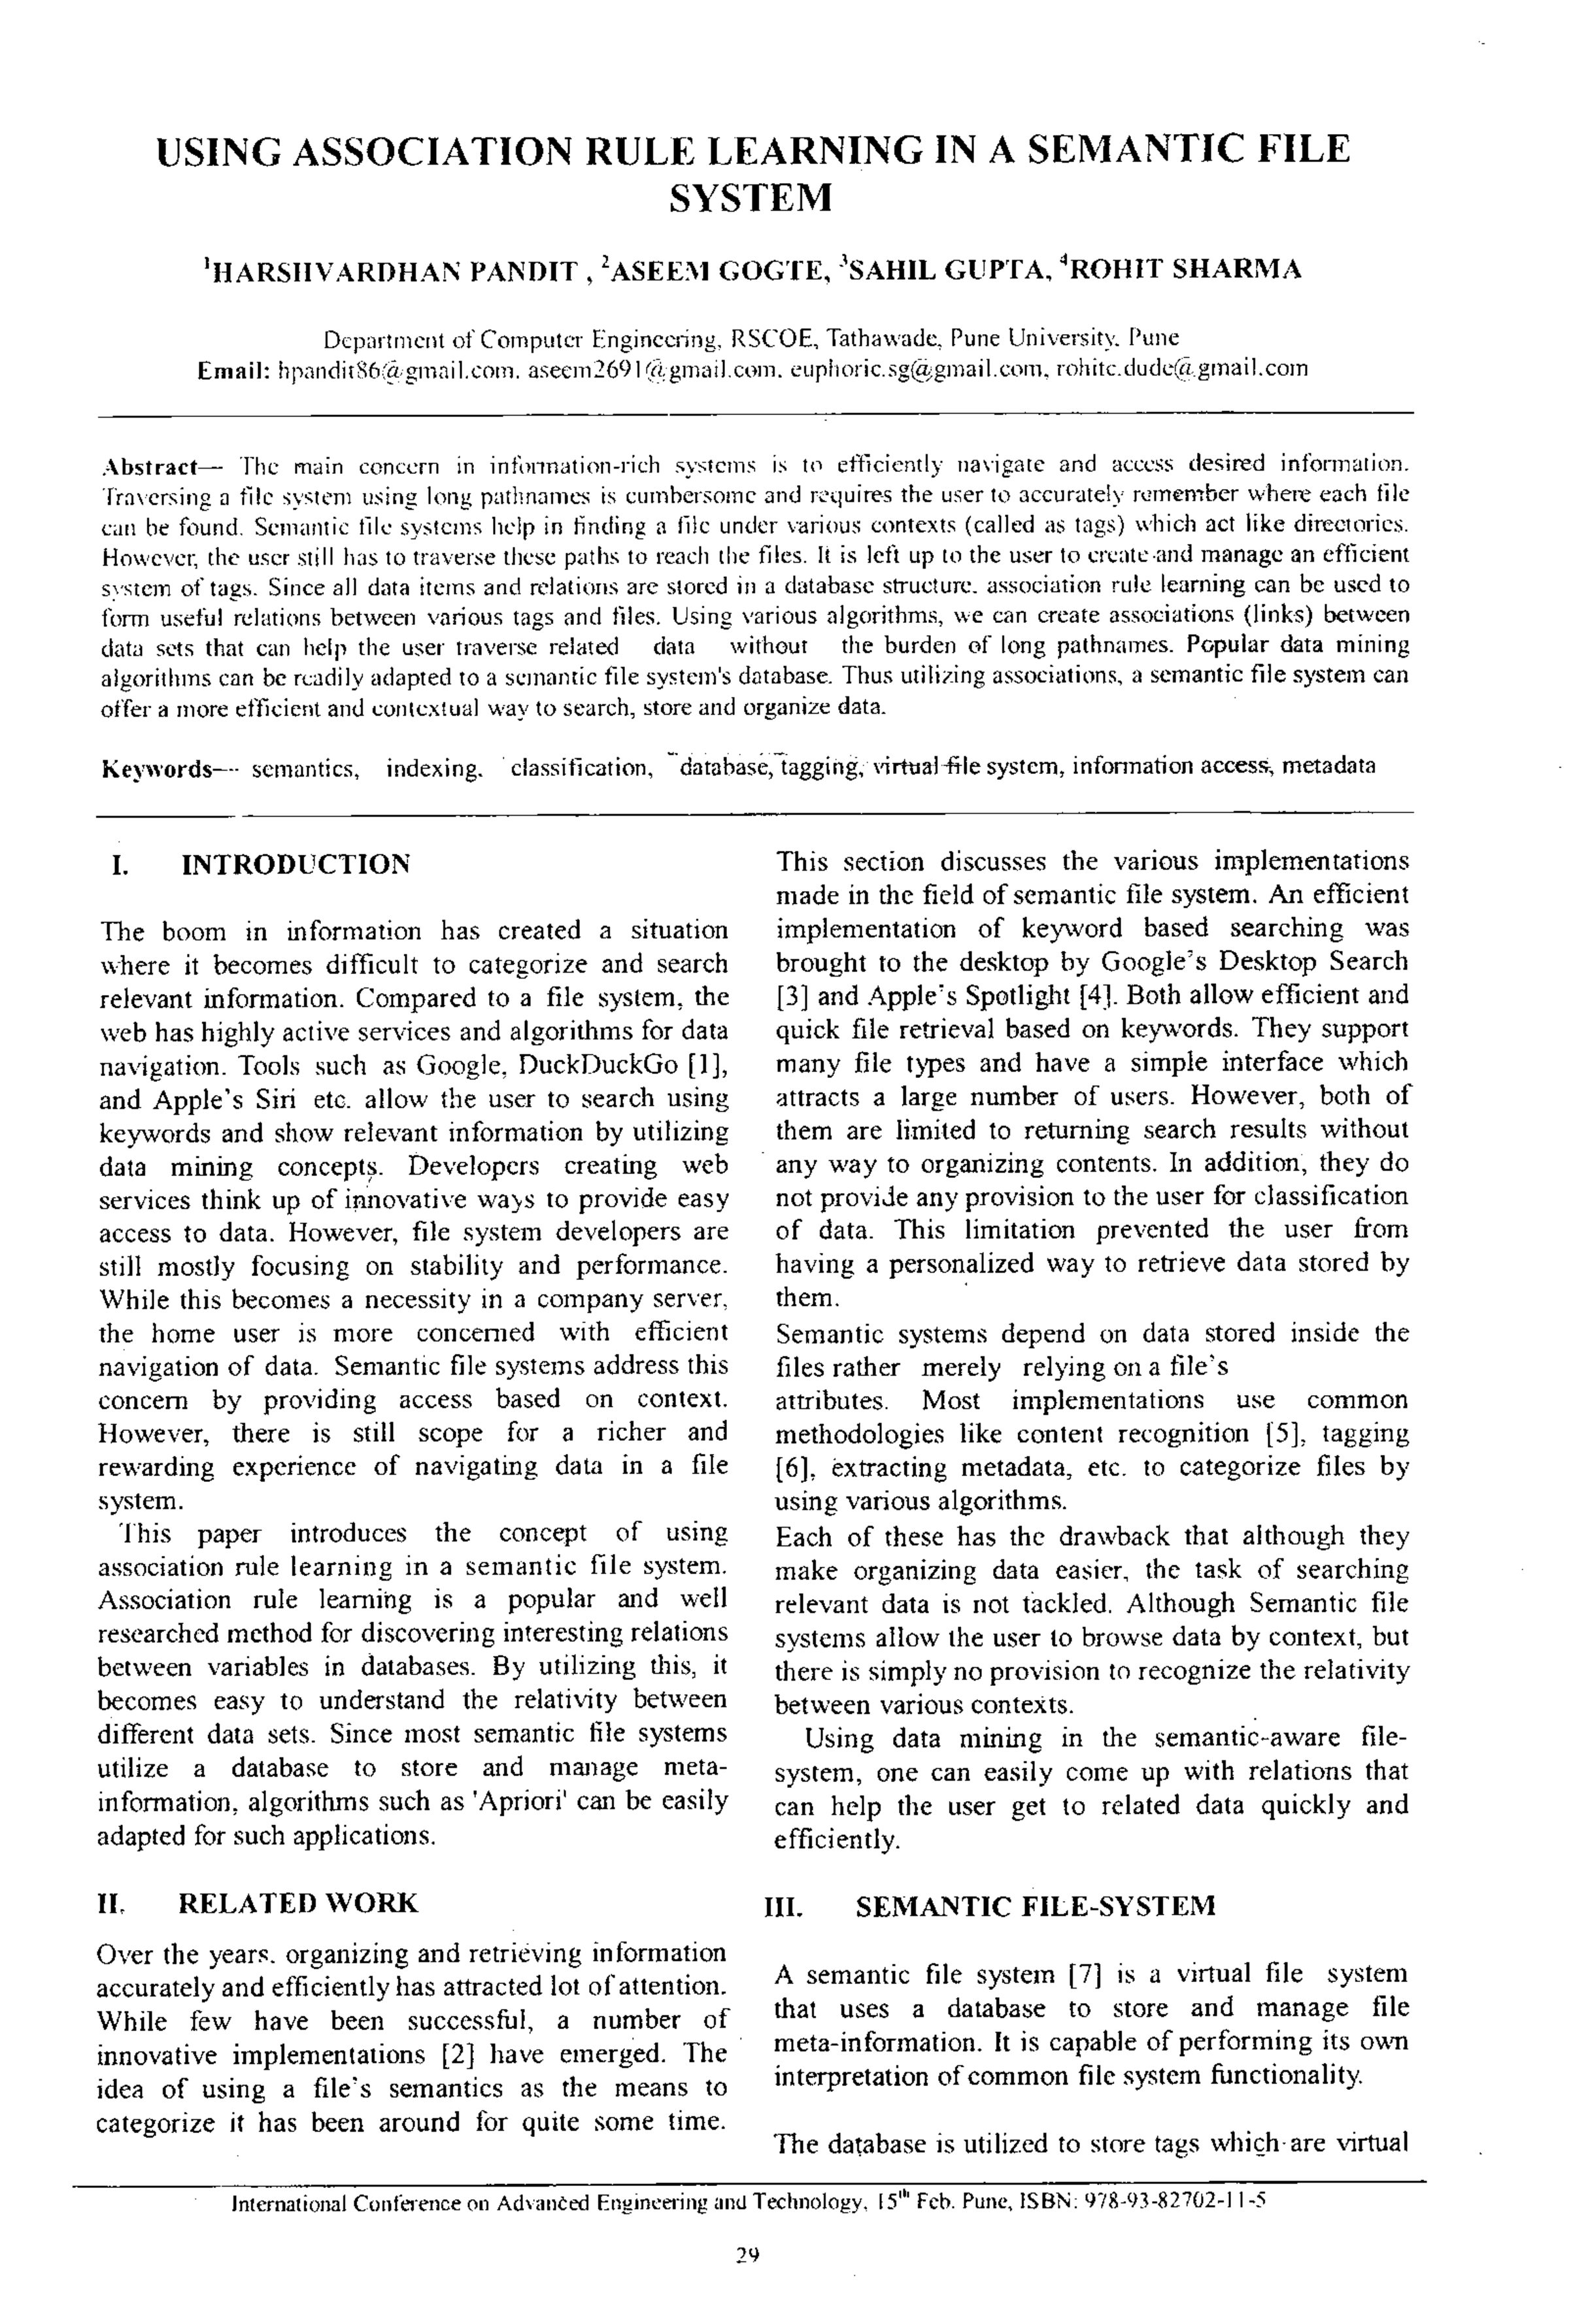
\includegraphics[page=1,scale=0.35]{./appendix/paperpage1.pdf}
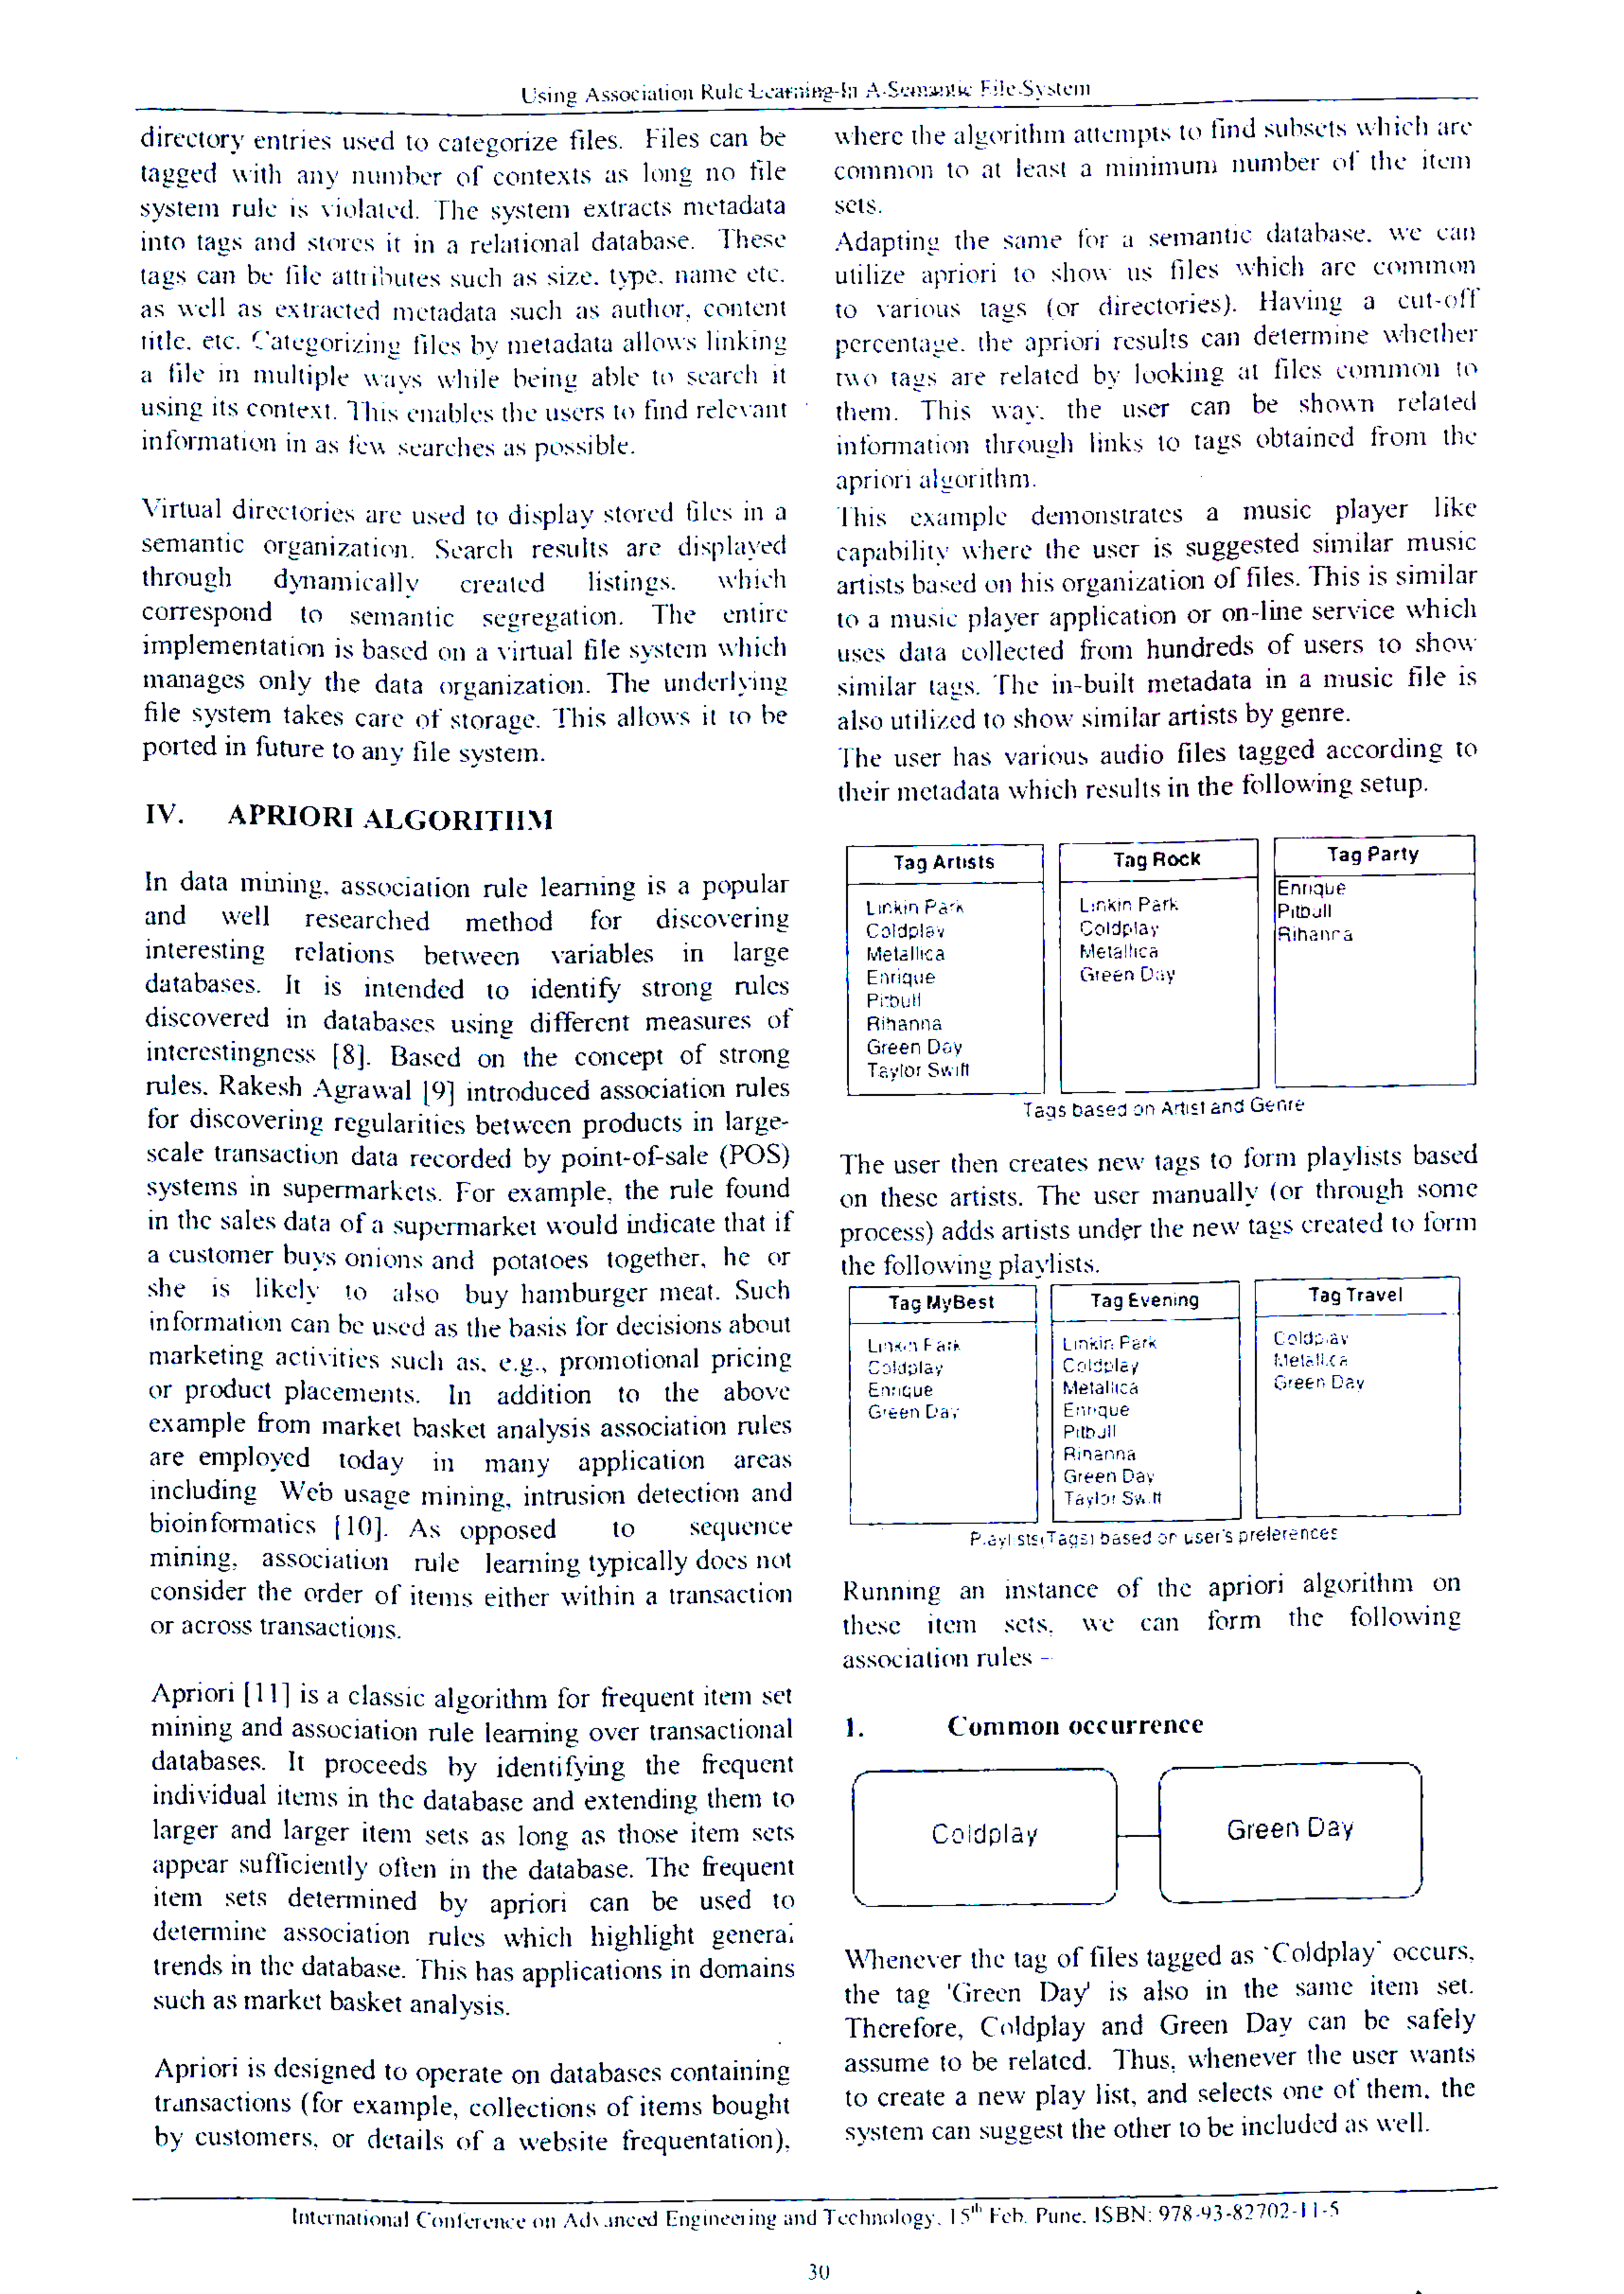
\includepdf[scale=0.85,pages=1-,offset=20 10,pagecommand={}]{./appendix/paperpage2.pdf}	
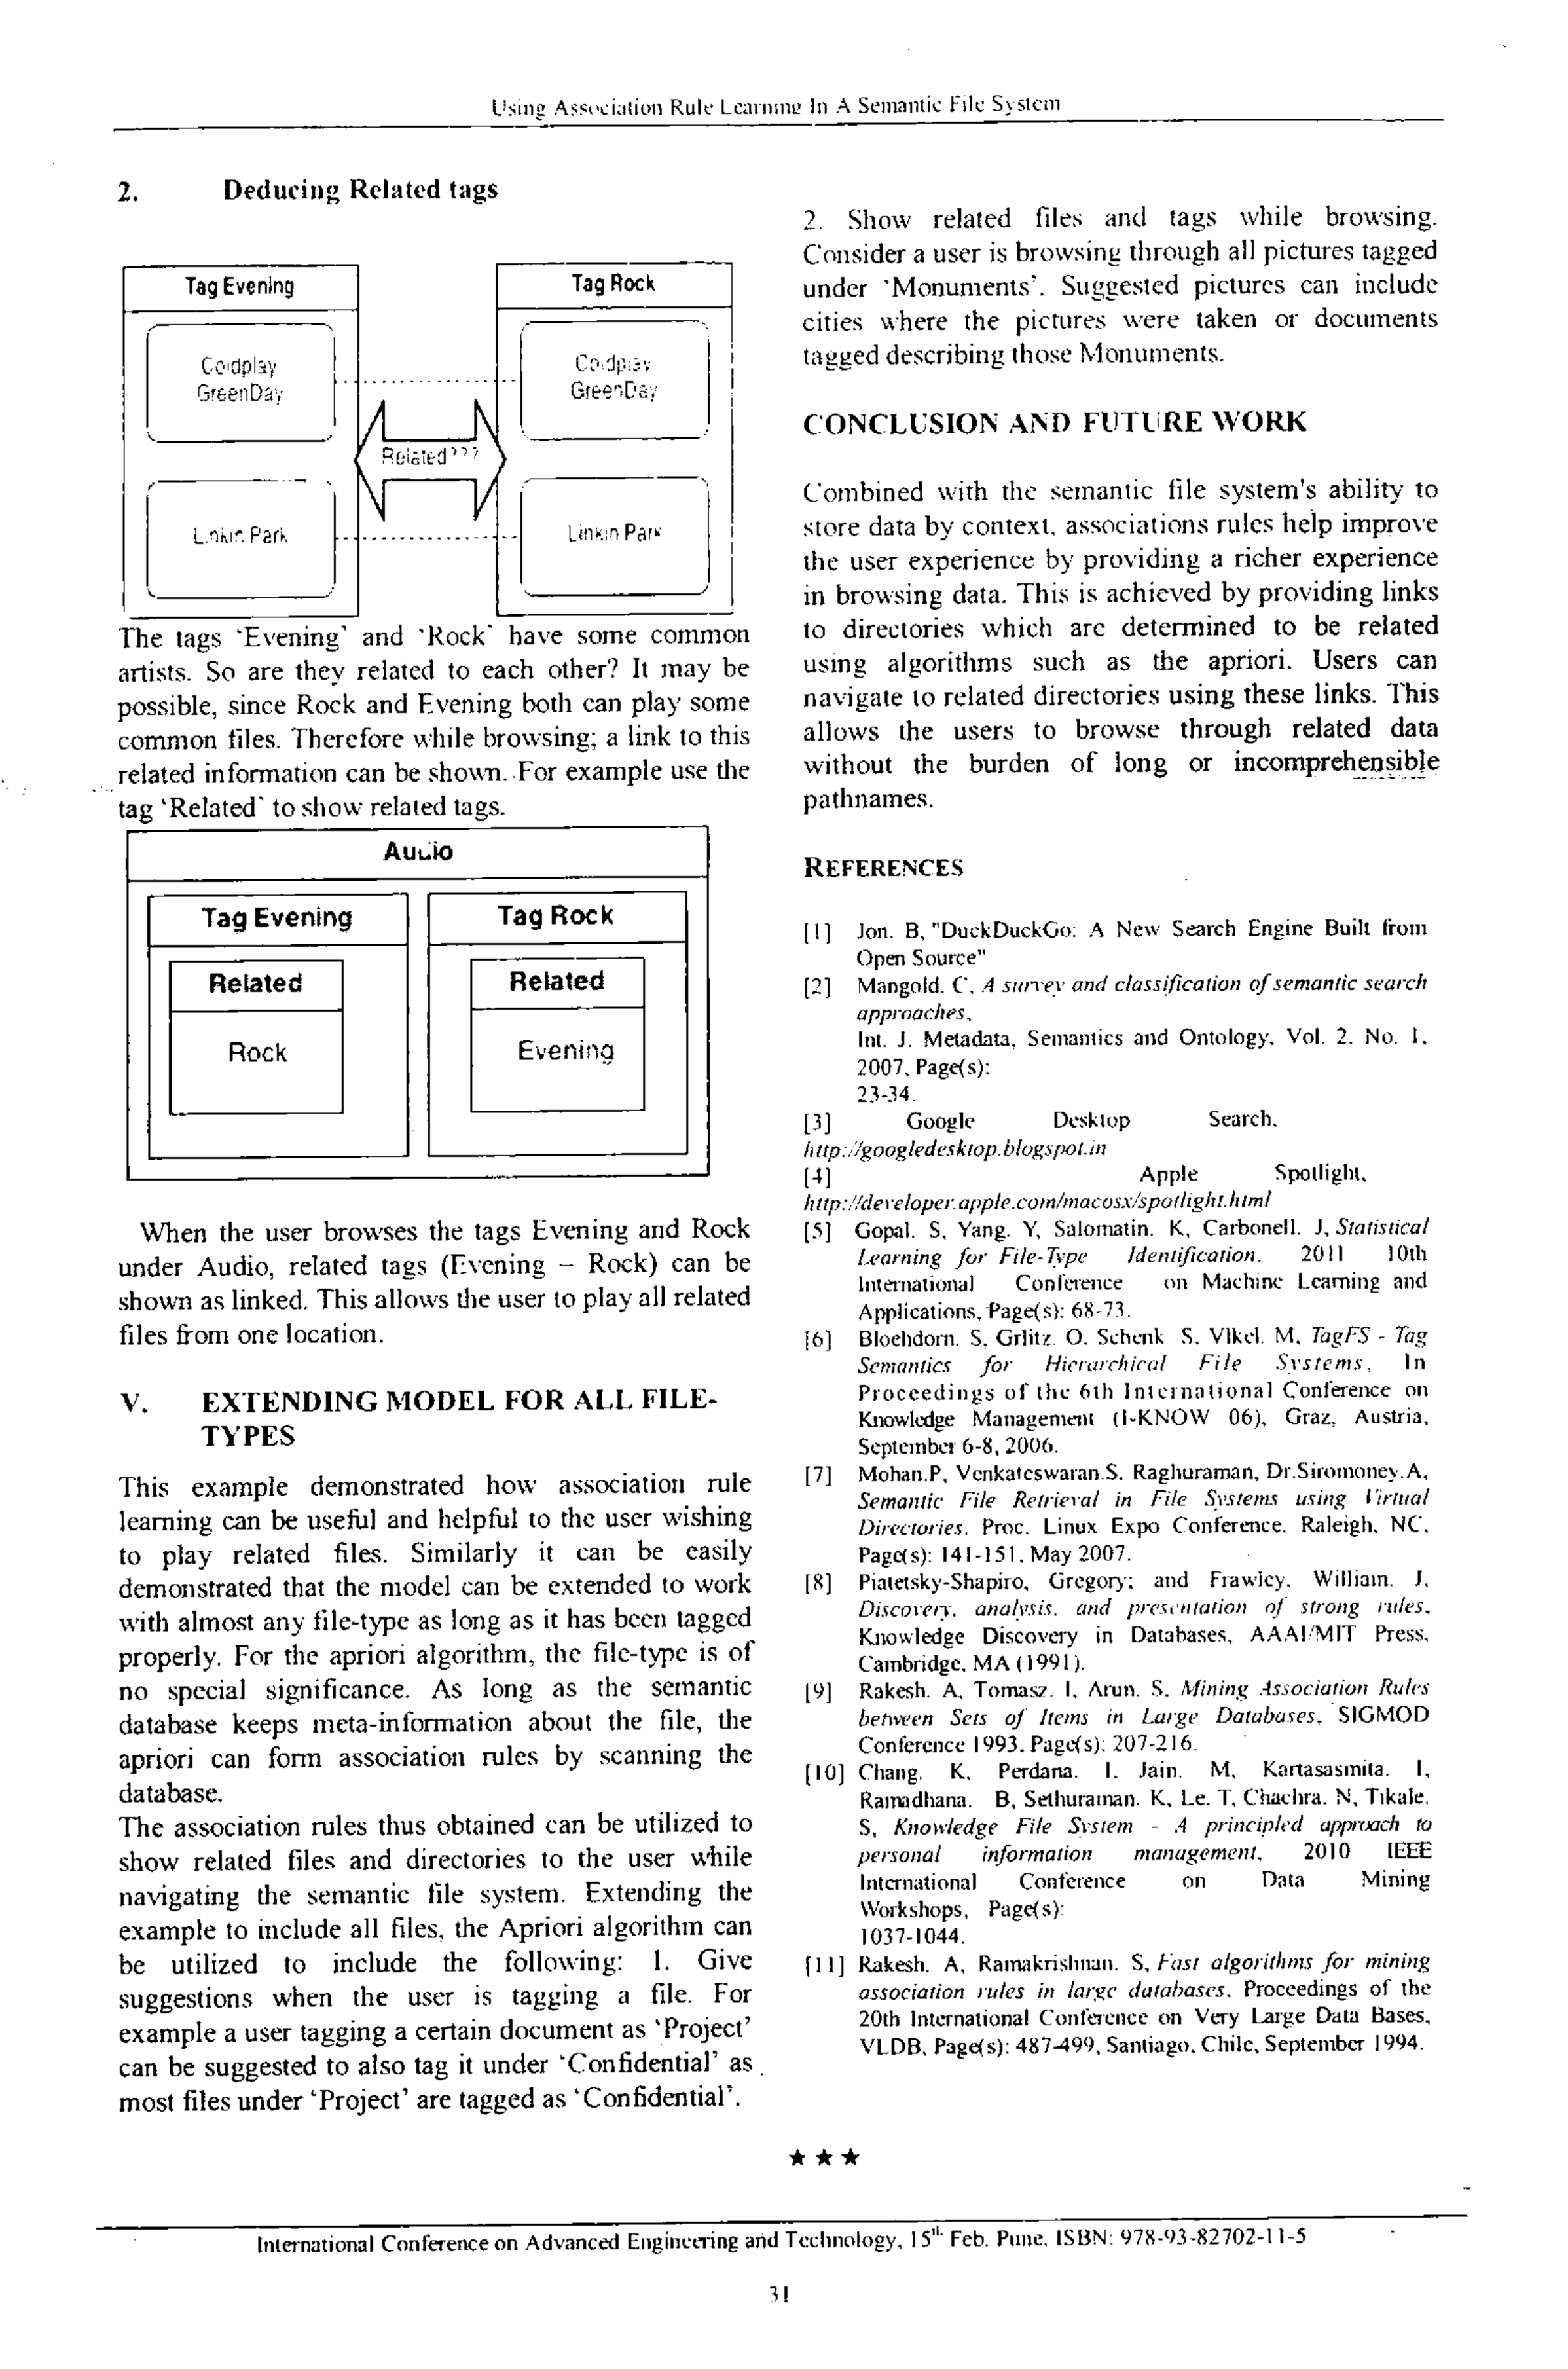
\includepdf[scale=0.85,pages=1-,offset=20 10,pagecommand={}]{./appendix/paperpage3.pdf}	

%\hspace*{-1.5cm}
\subsubsection{Reviewers comments:}
\begin{figure}[!h]
\centering
\setlength\fboxsep{0pt}
\setlength\fboxrule{0.5pt}
\fbox{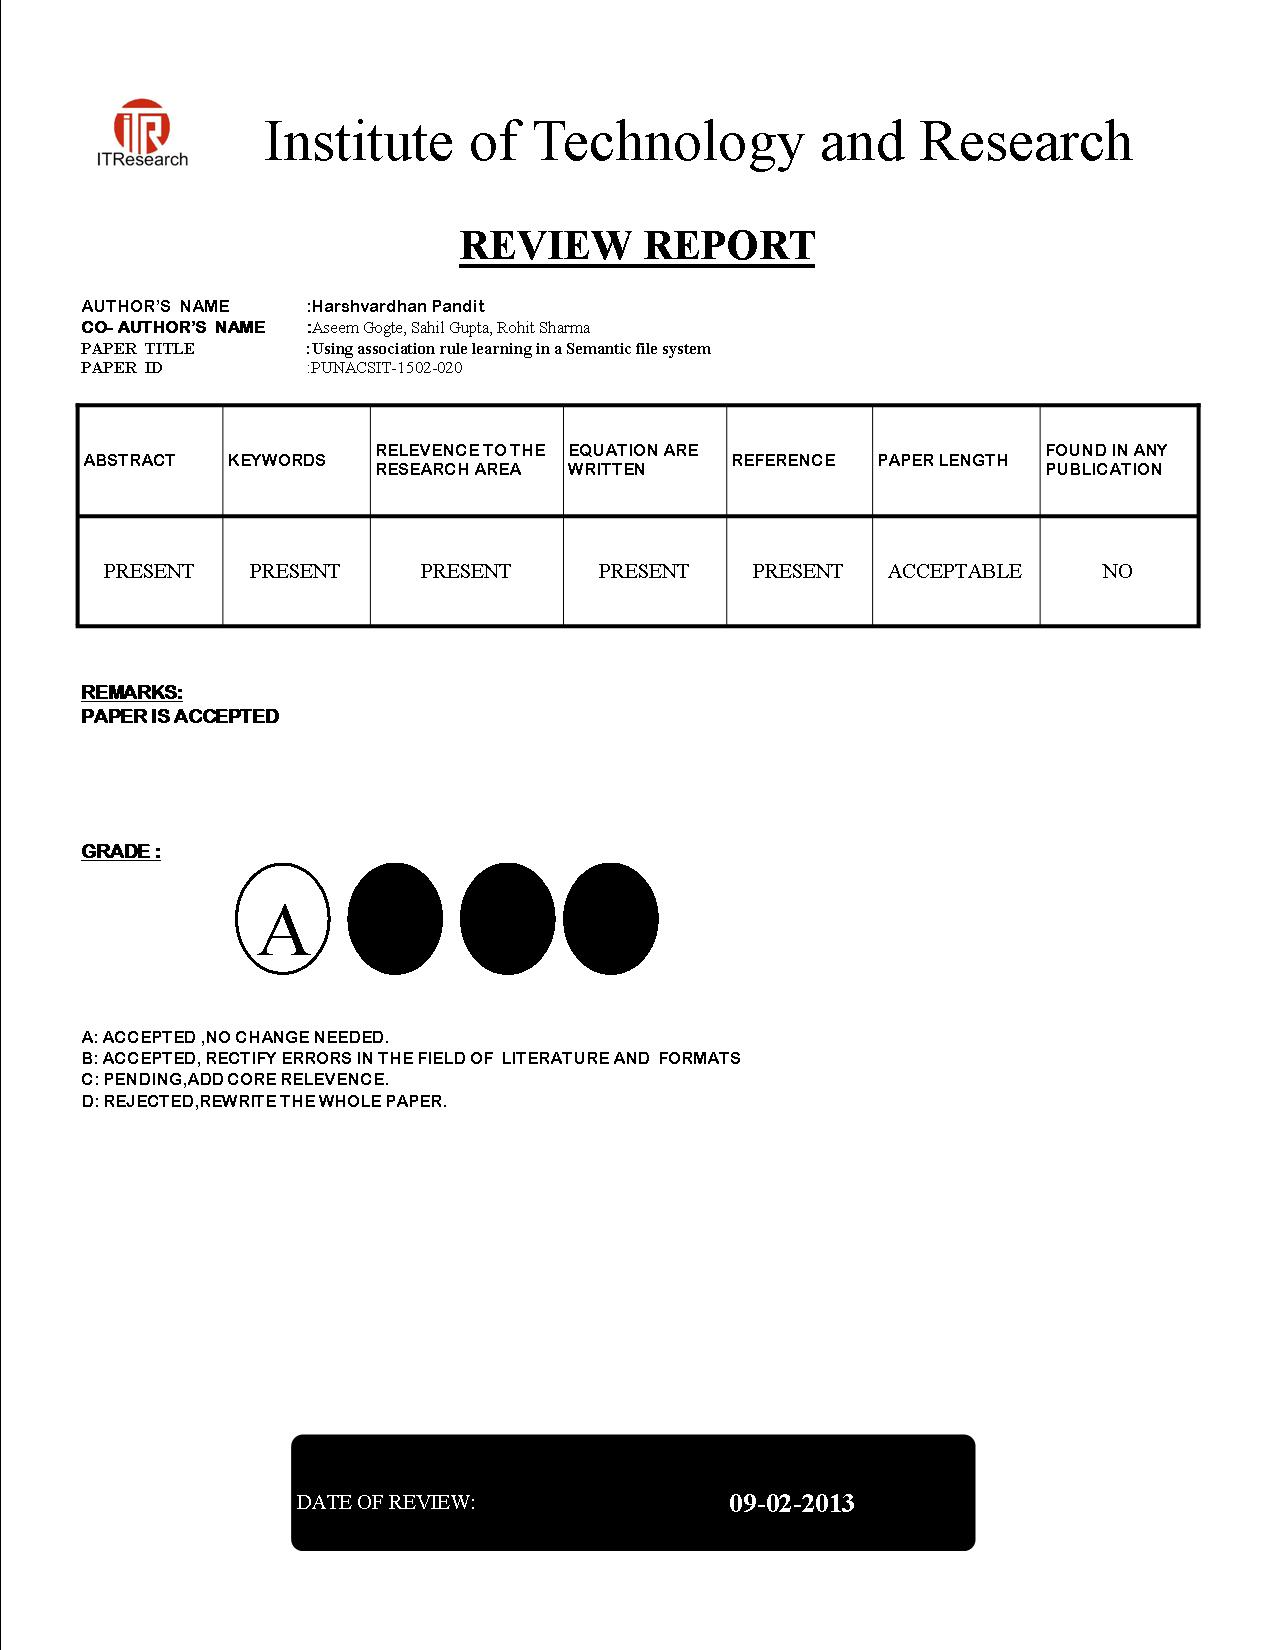
\includegraphics[width=0.8\linewidth]{./appendix/paper2review.jpg}}
%\includegraphics[width=0.8\textwidth]{image.png}
\caption{Reviewers comments}
\label{fig:RC1}
\end{figure}

\newpage
\subsection*{2.}

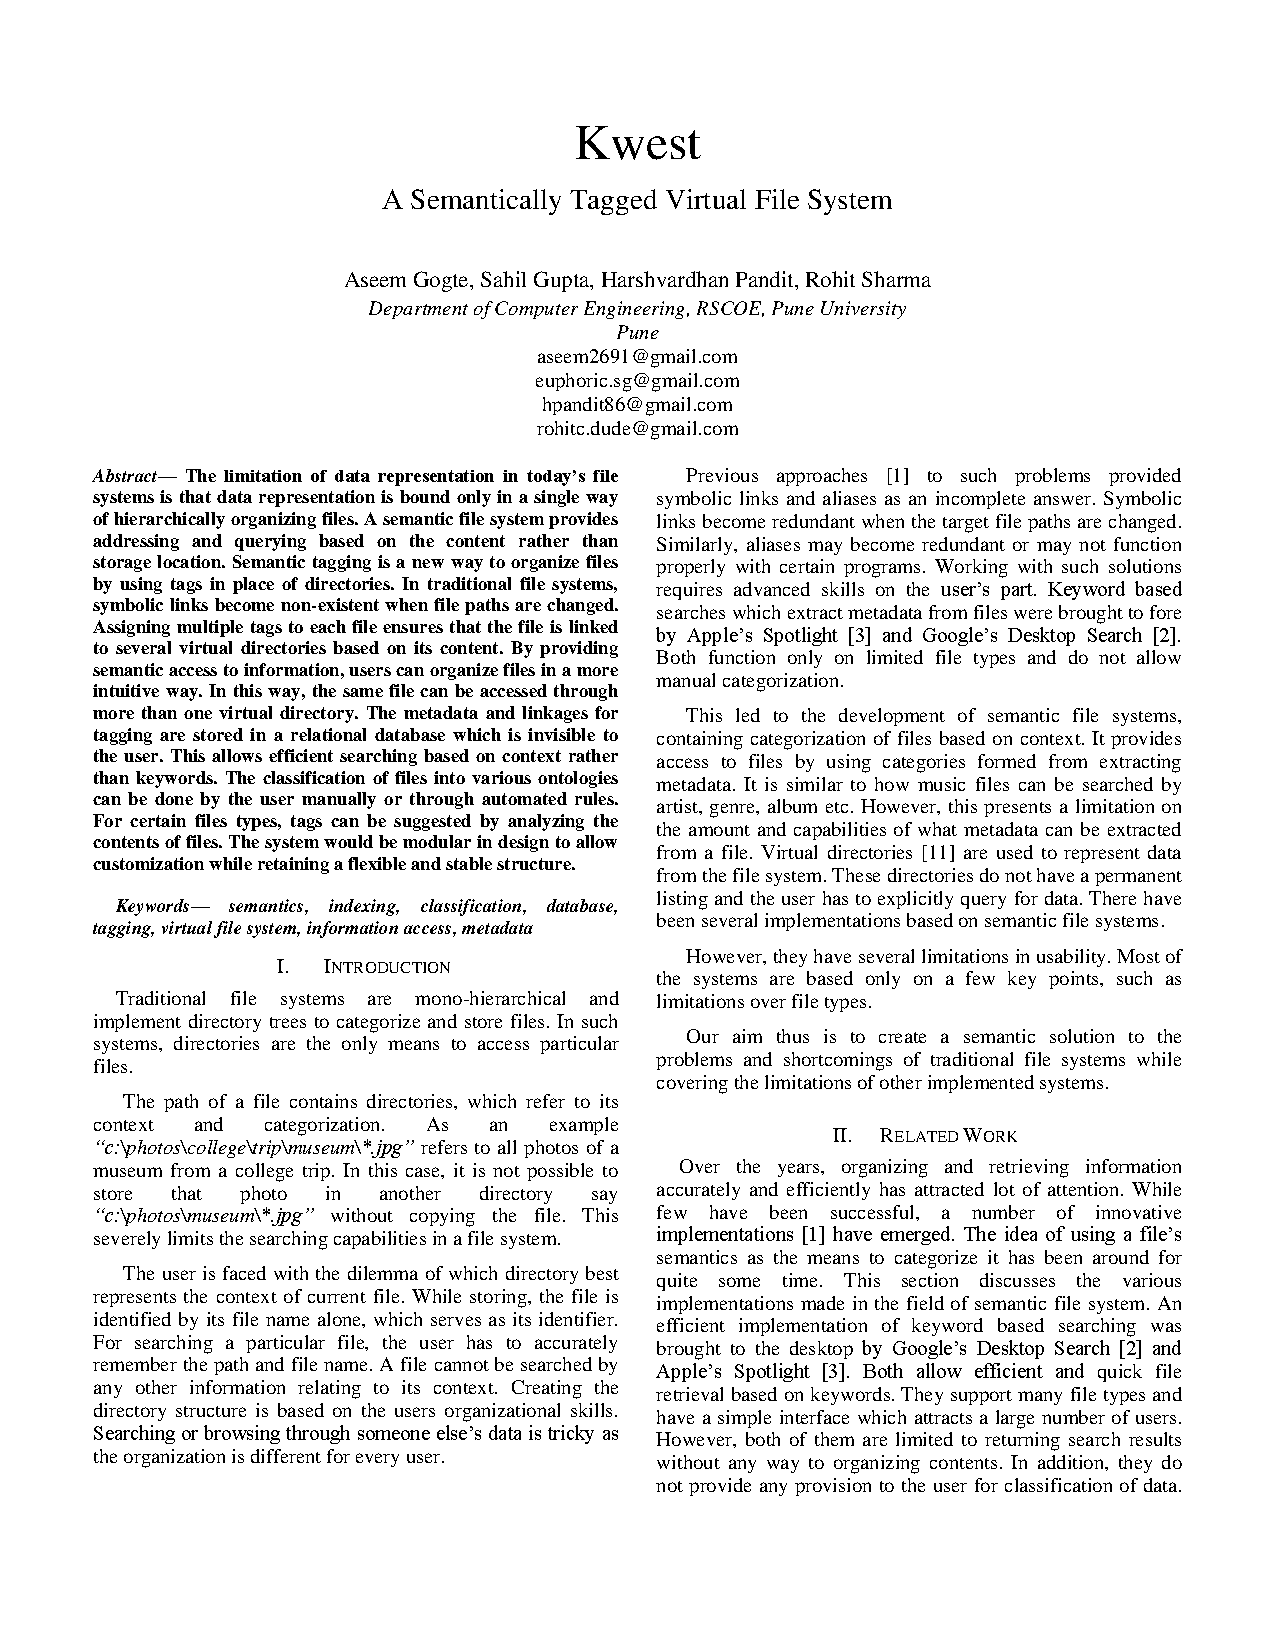
\includegraphics[page=1,scale=0.75]
{./appendix/sem1.pdf}
\includepdf[scale=0.85,pages=2-,offset=20 10,pagecommand={}]{./appendix/sem1.pdf}

\subsubsection{Reviewers comments:}
\begin{figure}[!h]
\centering
\setlength\fboxsep{0pt}
\setlength\fboxrule{0.5pt}
\fbox{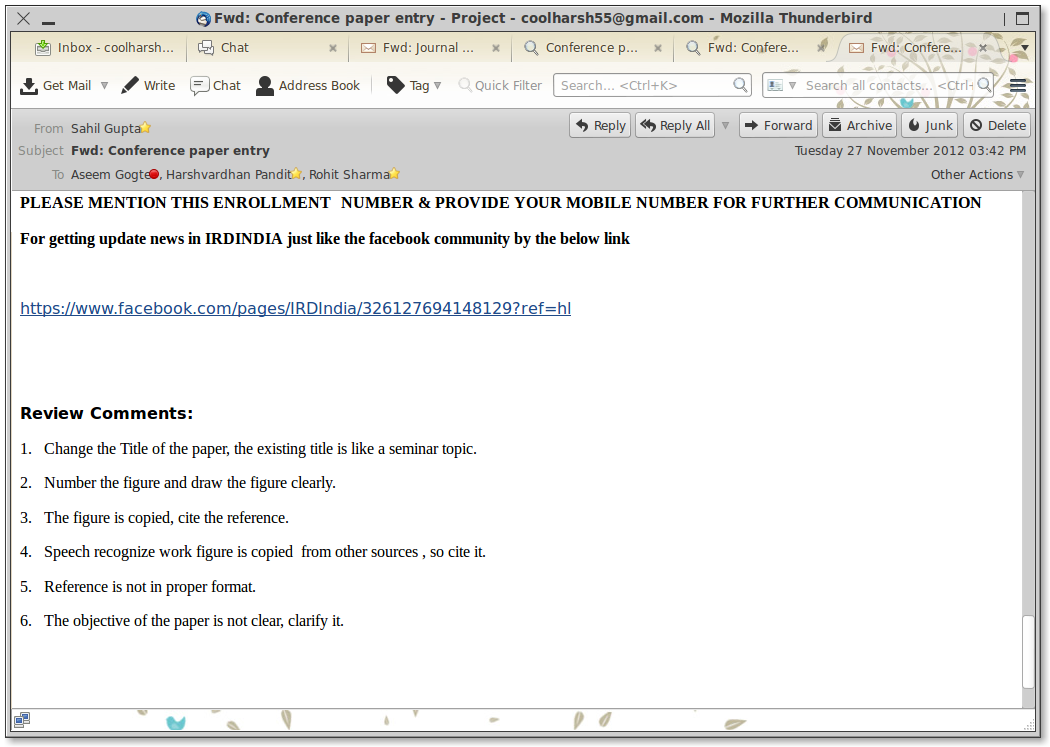
\includegraphics[width=0.8\linewidth]{./appendix/paper1review.png}}
%\includegraphics[width=0.8\textwidth]{image.png}
\caption{Reviewers comments}
\label{fig:RC2}
\end{figure}

\newpage
%\setcounter{section}{A}
\setcounter{subsection}{1}
\setcounter{subsubsection}{1}
\section*{APPENDIX D: PAPERS REFERRED}

\section{KFS - KNOWLEDGE FILE SYSTEM}
\hspace*{-1.5cm}
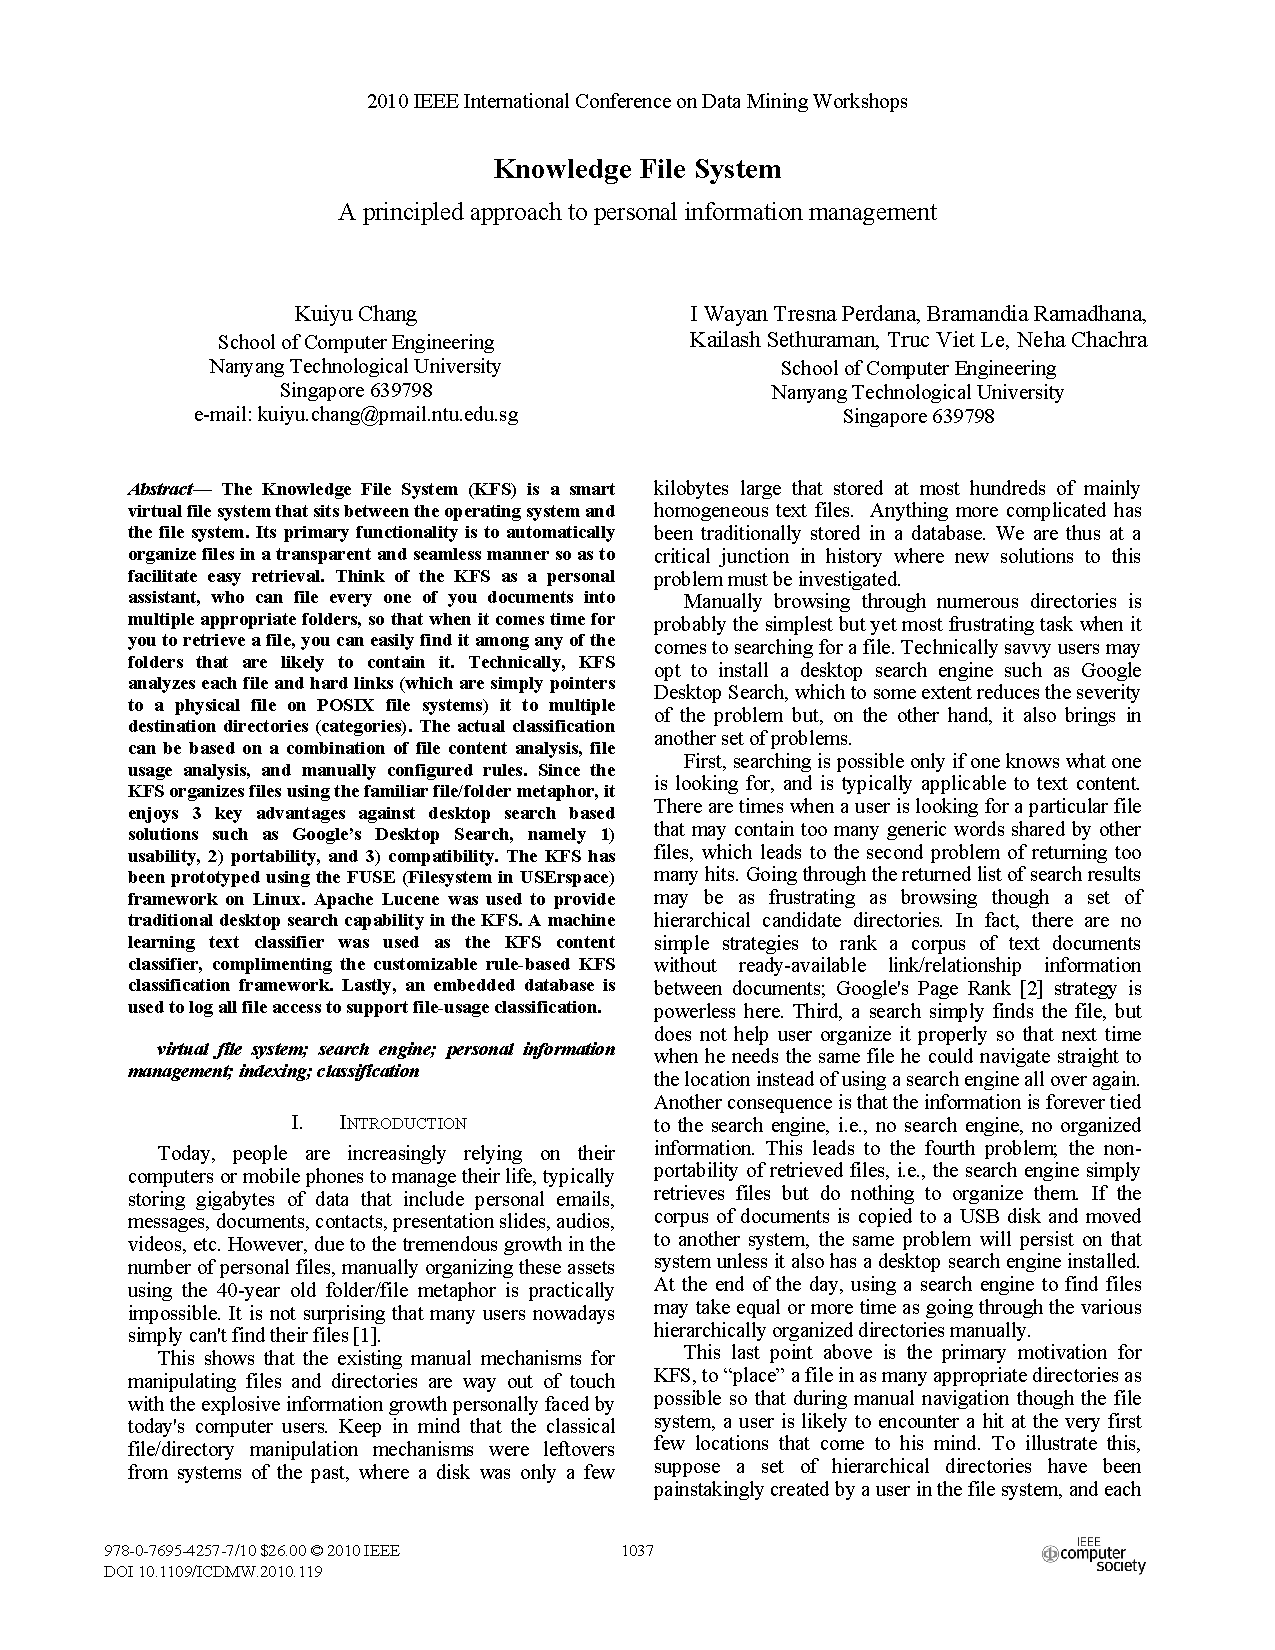
\includegraphics[page=1,scale=0.75]{./appendix/KFS.pdf}
\includepdf[scale=0.85,pages=2-,offset=20 10,pagecommand={}]{./appendix/KFS.pdf}


\section{Semantic-Aware Metadata Organization Paradigm in Next-Generation File Systems}
\hspace*{-1.5cm}
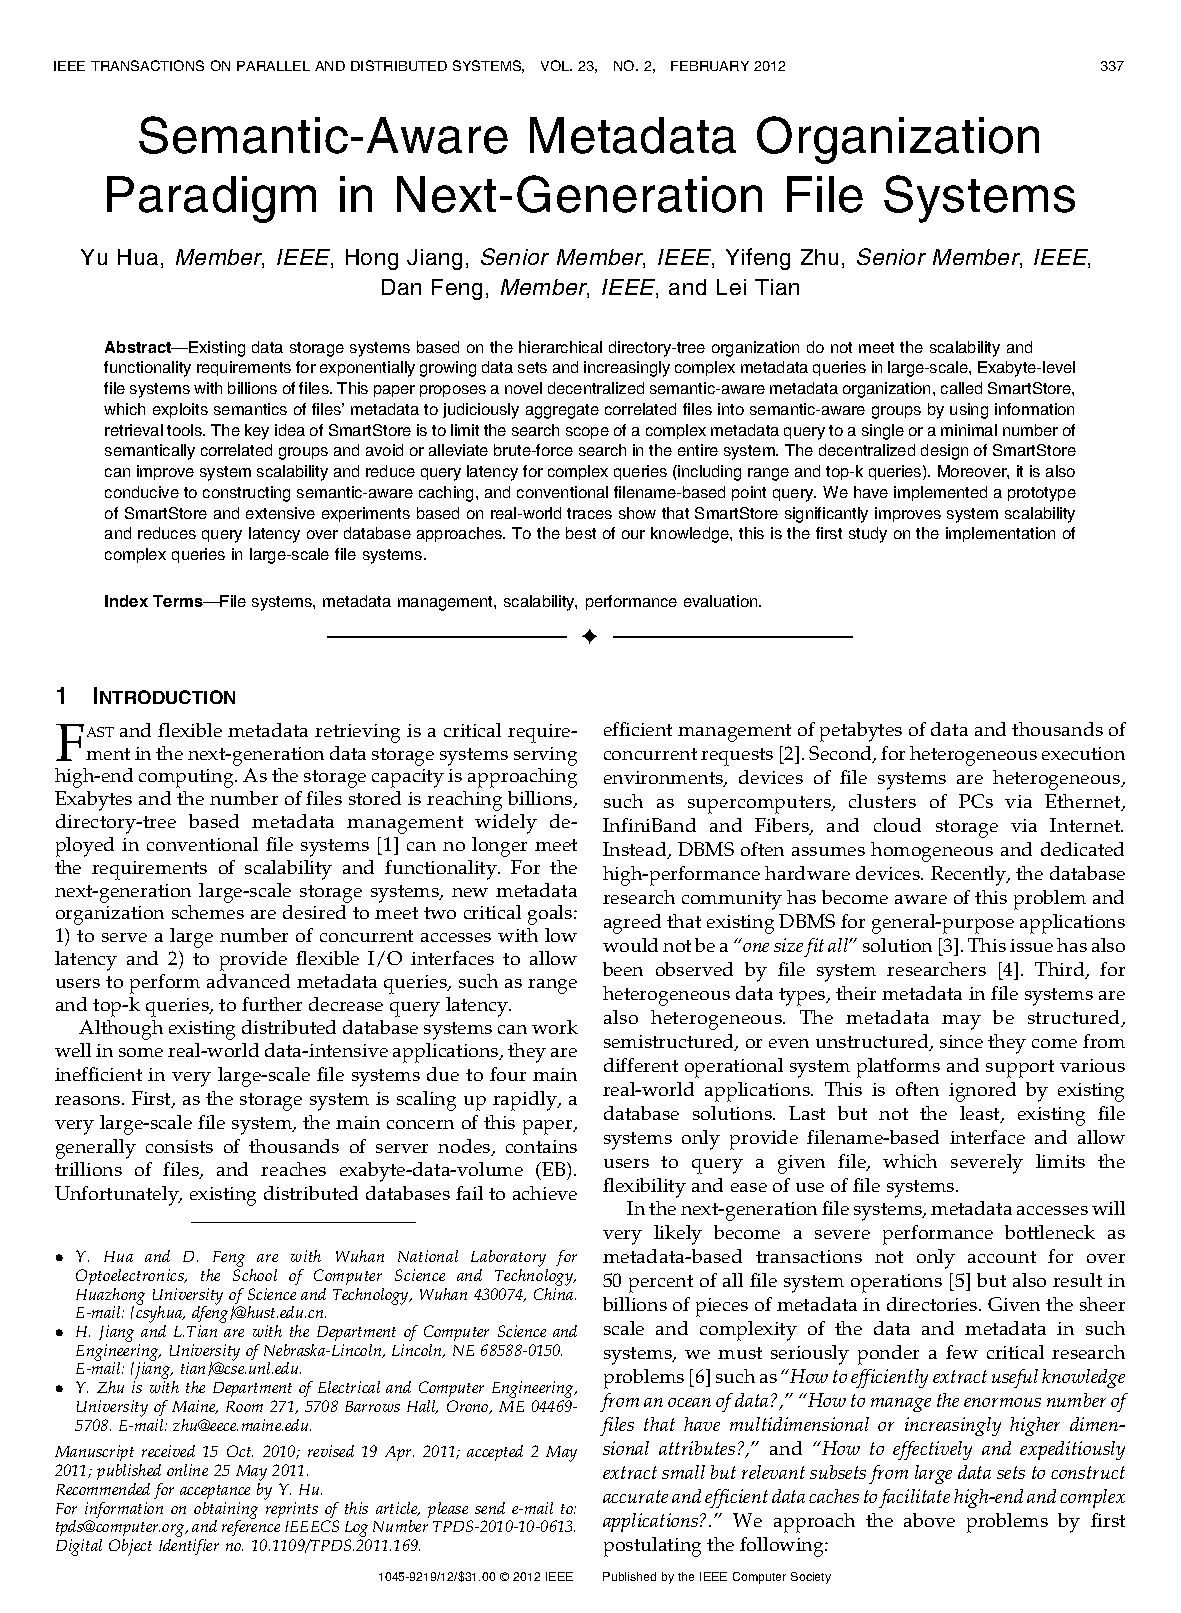
\includegraphics[page=1,scale=0.75]{./appendix/SM2012.pdf}
\includepdf[scale=0.85,pages=2-,offset=20 10,pagecommand={}]{./appendix/SM2012.pdf}	

\section{SEMANTIC FILE SYSTEM}
\hspace*{-1.5cm}
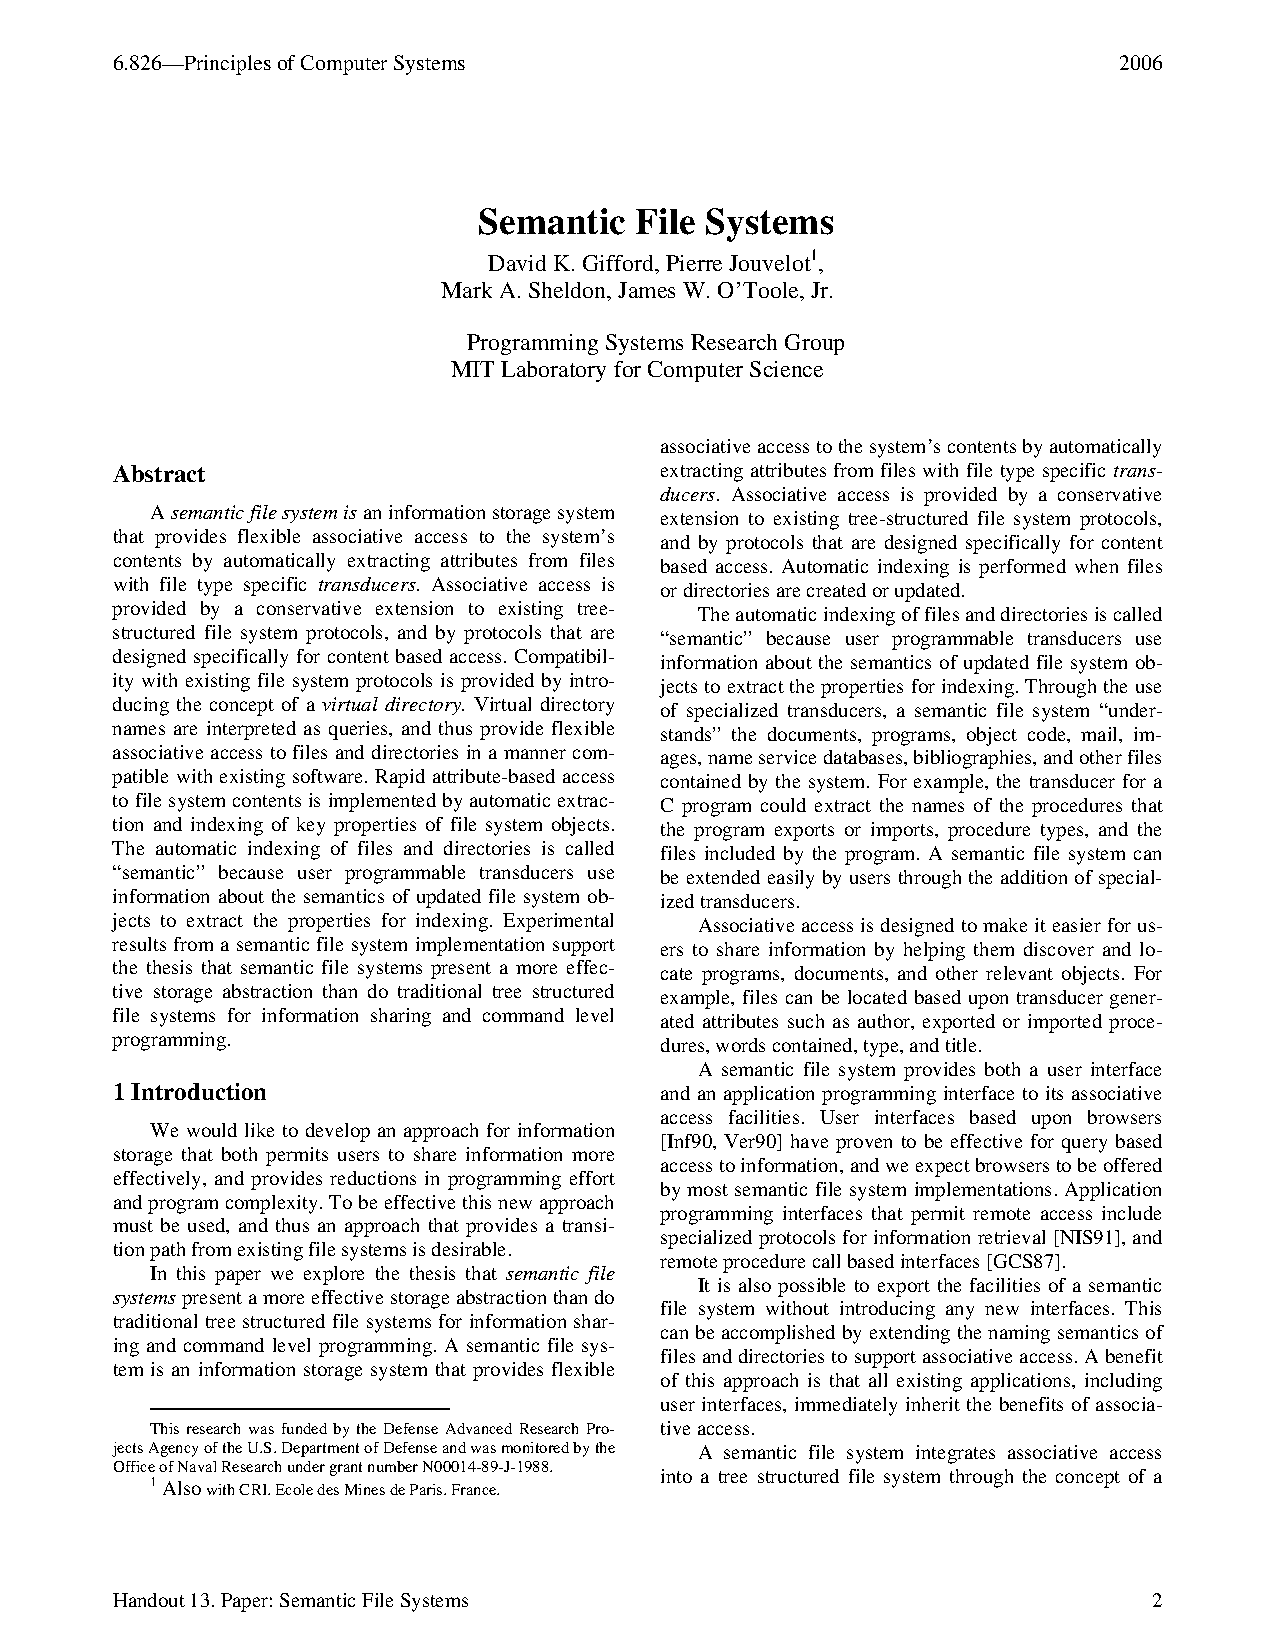
\includegraphics[page=1,scale=0.75]{./appendix/SEMFS.pdf}
\includepdf[scale=0.85,pages=2-,offset=20 10,pagecommand={}]{./appendix/SEMFS.pdf}



\newpage
%\setcounter{section}{0}
\setcounter{subsection}{1}
\setcounter{subsubsection}{1}
\section*{APPENDIX E : CONTRIBUTION OF TEAM MEMBERS} 
\emph{THIS SECTION IS A STUB. IS YET TO BE IMPLEMENTED...}
\noindent \textbf{Member 1: Aseem Gogte} 
\begin{itemize}
\item Mathematical Model
\item Testing related to Database 
\item Extraction of Metadata from Images \\
\end{itemize}

\noindent \textbf{Member 2: Sahil Gupta}
\begin{itemize}
\item Tag relations and behavior
\item Designing database queries
\item Database Design \\
\end{itemize}

\noindent \textbf {Member 3: Harshvardhan Pandit} 
\begin{itemize}
\item Interact with FUSE technology
\item Design Program flow
\item Component design \\
\end{itemize}

\noindent \textbf {Member 4: Rohit Sharma} 
\begin{itemize}
\item Extraction of Metadata from Audio / Video 
\item Database Design
\item Testing related to File operations
\end{itemize}



\newpage
%\setcounter{section}{0}
\setcounter{subsection}{1}
\setcounter{subsubsection}{1}
\chapter*{APPENDIX F: GLOSSARY}

\noindent \textbf{Acronyms} 
\begin{enumerate}
\item FUSE - File system in Userspace
\item GCC  - GNU Compiler Collection
\item GPL  - General Public License
\item API  - Application programming interface
\item GUI  - Graphical user interface
\item FAQ  - Frequently asked questions 
\item SFS  - Semantic File System
\item VFS  - Virtual File System
\item KFS  - Knowledge File System
\\
\end{enumerate}


\noindent \textbf{Term Definitions} \\
\begin{enumerate}
\item Semantic File System \\
Semantic File Systems are file systems used for information persistence which structure the data according to their semantics and intent, rather than the location as with current file systems. It allows the data to be addressed by their content (associative access) and querying for the data.
\item User Space \\
User space is that portion of system memory in which user processes run. This contrasts with kernel space, which is that portion of memory in which the kernel executes and provides its services.
\item File System \\
A 
file system 
is a 
means to 
organise 
data 
expected to be retained after a program 
terminates by providing procedures to store, retrieve and update data as well as 
manage the available space on the device(s) which contain it. 
\item Virtual File system \\
A virtual file system is an abstraction layer on top of a more concrete file system.
\item Virtual Directory \\
A virtual directory is a directory created in IIS to host our applications and to hide the actual physical location from the application users. 
It may simply designate a folder which appears in a path but which is not actually a sub-folder of the preceding folder in the path. 
\item Meta data \\
Metadata describes how and when and by whom a particular set of data was collected, and how the data is formatted.
\item Symbolic Links and Aliases \\
A symbolic link (also symlink or soft link) is a special type of file that contains a reference to another file or directory in the form of an absolute or relative path. 

%NEW NEW NEW NEW NEW NEW NEW NEW NEW NEW

\end{enumerate}




